Parallelism is increasingly seen as the only viable approach to
maintaining continued performance improvements in a multicore world.
Despite this, the adoption of parallel programming practises has been
slow and awkward, leading to a growing disparity between the levels of
available performance and the ability for application developers to
exploit it.

The multicore processors of modern devices offer many opportunities
for parallelism, but fully harnessing this processing power requires
an intimate knowledge of both the parallel programming semantics of
the language and performance characteristics of the underlying
hardware. In recent years, general purpose programming with GPUs
promises even greater data parallel throughput, but is a significantly
greater challenge to tame, forcing developers to master an unfamiliar
programming model (such as provided by CUDA or OpenCL) and
architecture (SIMD with a multi-level memory hierarchy). As such,
GPGPU programming is often considered beyond the realm of all but the
most expert of programmers. If steps are not taken to increase the
accessibility of such parallelism, this will only serve to widen the
gap between available and utilised performance as the core counts of
hardware continue to increase.

One possible solution for this \emph{programmability challenge} comes
in the form of algorithmic skeletons, which offer to simplify parallel
programming by raising the level of abstraction so that developers can
focus on solving problems, rather than coordinating parallel
resources. They achieve this by providing robust parallel
implementations of common patterns of computation which developers
parameterise with their application-specific code. This greatly
reduces the challenge of parallel programming, allowing users to
structure their problem solving logic sequentially, while offloading
the cognitive cost of parallel coordination to the skeleton author.


\section{Sacrificing Performance for Ease of Use}

Unfortunately, the performance of parallel programs is often sensitive
to low level parameter values, and when tuning these values, one size
\emph{cannot} fit all. The performance of parallel program parameters
are sensitive to the underlying hardware, to the program being
executed, and even to the \emph{dataset} that is operated upon. This
is especially problematic for algorithmic skeletons, as skeleton
authors cannot tune the performance of an implementation across the
breadth of these three dimensions, and this results in programs which
forgo the performance advantages that can be achieved with the low
level tuning of hand written parallel code.


% First prong: standardise autotuning

If the performance of algorithmic skeletons is to be competitive with
that of hand crafted parallel programs, then these skeletons must be
capable of adapting to their environments. The development of such
\emph{autotuning} software is an entire research field itself --- and
understandably so: there is an irresistible appeal to the idea of
software which is capable of improving its own efficiency without the
need for human intervention. The unfortunate reality is that while
these autotuning systems share the unified goal of improving the
performance of their respective optimisation targets, the range of
competing approaches and implementations has resulted in a fragmented
state in which no one system has been able to gain the critical mass
to achieve mainstream traction.

This is the first aim of this thesis: to tackle the issue of providing
a unified interface for autotuning which reduces the amount of
redundant and overlapping work needed to implement autotuning for
different optimisation targets.

% Second prong: machine learning to cut down cost

The second aim of this thesis is to explore techniques for predictive,
machine learning-enabled autotuning for use in algorithmic
skeletons. Typically, autotuning using iterative compilation requires
enumerating some portion of the optimisation space for each program
being tuned; however, the cost of such an exploration is prohibitively
expensive when summed across the broad range of use cases targeted by
algorithmic skeletons. As such, successfully autotuning algorithmic
skeletons will require a method for \emph{predicting} the values of
parameters which will maximise performance, without the need for trial
and error. To succeed, such a method of tuning does not need to
provide perfectly accurate predictions, but simply sufficiently
performant results so that, when combined with the vast accessibility
improvements offered by algorithmic skeletons, it provides a
convincing argument for algorithmic skeletons as the solution to the
parallel programmability crisis.


\section{Contributions}

The key contributions of this thesis are:

\begin{itemize}
\item The development of \emph{OmniTune} --- a novel and extensible
  framework for the collaborative autotuning of optimisation
  parameters across the life cycle of programs.
\item The application of OmniTune for tuning of the SkelCL algorithmic
  skeleton library. When tasked with predicting the workgroup sizes of
  stencil skeletons on both GPUs and CPUs, OmniTune achieves 94\% of
  the available performance, providing a median speedup of
  $1.33\times$ over values predicted by human experts, or $3.79\times$
  over the best possible statically chosen parameter values.
\item The novel application of procedurally generated benchmark
  programs for training machine learning-enabled autotuners. This
  reduces the cost of training while increasing the size of the space
  which can be explored. The effectiveness of this approach is
  demonstrated by testing the OmniTune SkelCL autotuner trained using
  synthetic benchmarks against 68 configurations of real world stencil
  kernels, achieving comparable autotuning performance with that of
  cross-validation.
\item An empirical evaluation of the performance of workgroup size to
  parameterise high-level parallel patterns. I enumerate the
  optimisation space of workgroup sizes for SkelCL stencil kernels
  across 269813 test cases, demonstrating an average performance loss
  of up to $15.14\times$ if workgroup size is not correctly tuned.
\item A comparison of multiple approaches for runtime autotuning:
  using classifiers to predict optimal parameter values, using
  regressors to predict the absolute runtime of programs, and using
  regressors to predict the relative performance of different
  parameter values.
\end{itemize}


\section{Motivation}

\begin{figure}
\centering
\begin{subfigure}[h]{.49\textwidth}
\centering
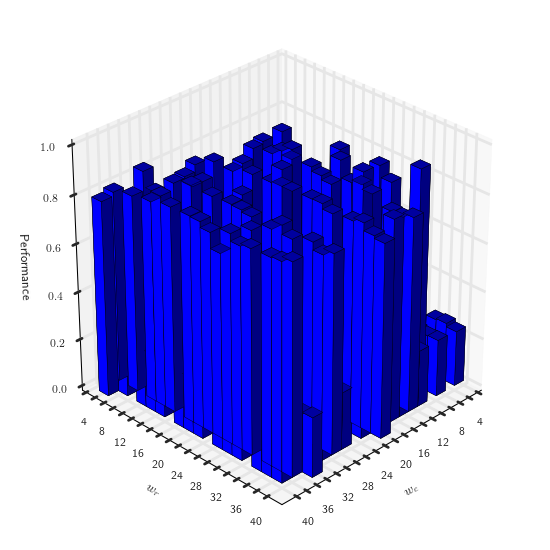
\includegraphics[width=1.0\textwidth]{img/motivation_1}
\vspace{-1.5em} % Shrink vertical padding
\caption{}
\label{fig:motivation-1}
\end{subfigure}
~%
\begin{subfigure}[h]{.49\textwidth}
\centering
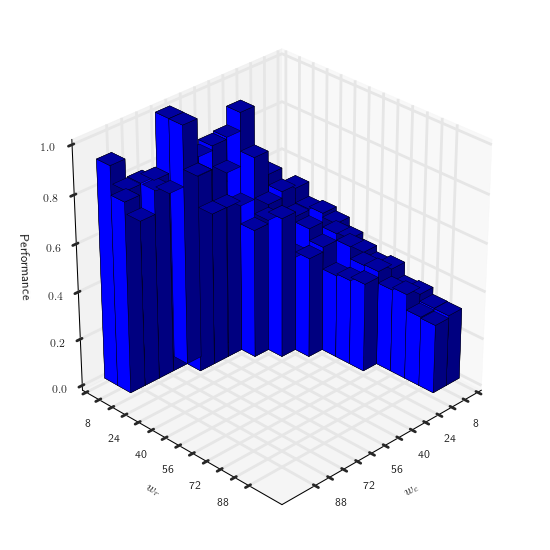
\includegraphics[width=1.0\textwidth]{img/motivation_2}
\vspace{-1.5em} % Shrink vertical padding
\caption{}
\label{fig:motivation-2}
\end{subfigure}
\caption[Workgroup size optimisation space across devices]{%
  Workgroup size optimisation space of a stencil benchmark across
  devices: (\subref{fig:motivation-1}) Intel CPU,
  (\subref{fig:motivation-2}) NVIDIA GPU. This shows that stencil
  performance is dependent on properties of the underlying
  architecture, with different optimal workgroup sizes ($56 \times 20$
  vs.\ $64 \times 4$) for the two devices shown.%
}
\label{fig:motivation-arch}
\end{figure}

\begin{figure}
\begin{subfigure}[h]{.49\textwidth}
\centering
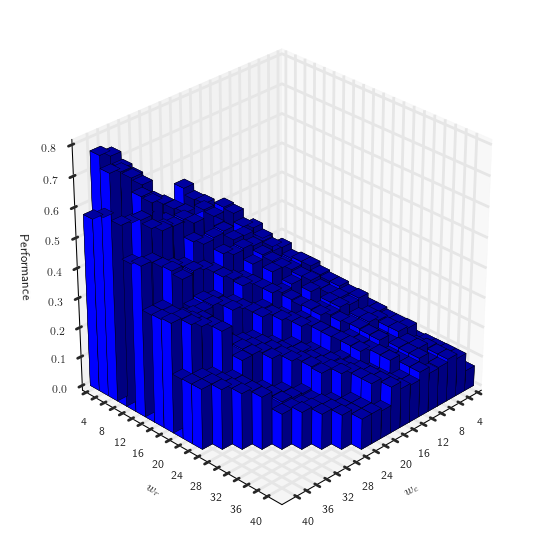
\includegraphics[width=1.0\textwidth]{img/motivation_3}
\vspace{-1.5em} % Shrink vertical padding
\caption{}
\label{fig:motivation-3}
\end{subfigure}
~%
\begin{subfigure}[h]{.49\textwidth}
\centering
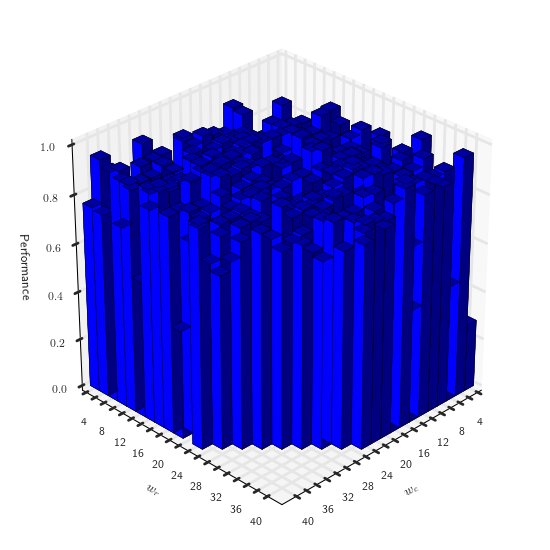
\includegraphics[width=1.0\textwidth]{img/motivation_4}
\vspace{-1.5em} % Shrink vertical padding
\caption{}
\label{fig:motivation-4}
\end{subfigure}
\caption[Workgroup size optimisation space across stencils]{%
  Workgroup size optimisation space of two stencils on the same
  device. Despite the underlying hardware being the same, the relative
  performance of workgroup sizes varies greatly between the two
  programs. The optimal workgroup sizes are $128\times2$ and
  $256\times4$ respectively.%
}
\label{fig:motivation-prog}
\end{figure}

In this section I present the case for autotuning the workgroup size
of SkelCL stencil skeletons. Stencil workgroup sizes presents a two
dimensional parameter space, consisting of a number of rows and
columns. It is constrained by properties of both the stencil code and
underlying architecture. For a detailed discussion of the parameter
space and experimental methodology, see Chapters~\ref{chap:background}
and~\ref{chap:methodology}.

By comparing the mean runtime of a stencil program using different
workgroup sizes while keeping all other conditions constant, we can
assess the relative performance of different points in the
optimisation space. Plotting this two dimensional optimisation space
using a three dimensional bar chart provides a quick visual overview
of the optimisation space. The two horizontal axes are used to
represent the number of rows and columns in a workgroup, while the
height of each bar shows the performance of a program at that point in
the space (higher is better).

If the performance of workgroup sizes were not dependent on the
execution device, we would expect the relative performance of points
in the optimisation space to be consistent across devices. As shown in
Figure~\ref{fig:motivation-arch}, this is not the case, with the
optimisation space of the same benchmark on different devices being
radically different. Not only does the optimal workgroup size change
between devices, but the performance of suboptimal workgroup sizes is
equally dissimilar.

The optimisation space of~\ref{fig:motivation-1} has a grid-like
structure, with clear performance advantages of workgroup sizes at
multiples of 8 columns. A developer specifically targeting this device
would learn to select workgroup sizes which follow this pattern. This
domain specific knowledge does not transfer to the device shown
in~\ref{fig:motivation-2}, where the relatively simple optimisation
space is more amenable to a stochastic hill climbing search.

Similarly, the optimisation space of two different stencils on the
same device is shown in~\ref{fig:motivation-prog}, demonstrating that
the optimisation space is dependent on the program being executed.

The optimal workgroup size is different for each of the four examples,
and the difference between the maximum and minimum performance
workgroup sizes provides an average $37.0\times$ speedup. The existing
SkelCL stencil implementation uses a statically chosen workgroup size
of $32\times4$, and this provides an average of only 63\% of the
available performance when compared to the best workgroup size for
these four examples. Even for this small set of examples, static
values and simple heuristics cannot provide portable performance. The
workgroup size parameter is sensitive to factors outside the influence
of the developers control, such as the type of program, the data being
operated on, and the execution device. This makes portable performance
tuning a difficult task, and it has traditionally been the
responsibility to domain specialists to laboriously hand tune
individual programs to match the target problem and underlying
hardware.

Given the important role that stencil codes play in many fields of
computer science and simulation, and the difficulties in selecting
workgroup sizes for portable performance, I believe that there is a
compelling case for the development of an autotuner which can
accommodate for these differences of workgroup size performance
between devices and programs. It is my hypothesis that the performance
of algorithmic skeletons will be improved by developing an autotuner
which considers dynamic features which cannot be determined at compile
time. The premise is that the optimisation spaces of algorithmic
skeletons such as stencils are shaped by features which can only be
determined at runtime. Effective searching of these spaces can only be
performed by collecting empirical data rather than building predictive
models.

The ambition of this thesis is to demonstrate that, using machine
learning, we can develop predictive tuning systems which closely
approach --- and in some cases, outperform --- the kinds of ad-hoc
hand tuning which traditionally came at the cost of many man hours of
work from expert programmers to develop.


\section{Structure}

The remainder of the document is structured as follows:
%
\begin{itemize}
\item Chapter~\ref{chap:background} contains necessary background
  material, an introduction to the SkelCL framework, and a description
  of the techniques used throughout the thesis;
\item Chapter~\ref{chap:related} contains an exposition of relevant
  literature in the field of autotuning and heterogeneous parallelism,
  contrasting the related research with my own;
\item Chapter~\ref{chap:autotune} presents OmniTune, an extensible and
  distributed autotuner capable of predicting optimisation parameter
  values for unseen programs and devices at runtime;
\item Chapter~\ref{chap:omnitune-skelcl} describes the application of
  OmniTune for selecting the workgroup size of SkelCL stencils;
\item Chapter~\ref{chap:methodology} describes a comprehensive
  exploration of the workgroup size optimisation space for stencil
  skeletons, including the methodology for obtaining performance data
  and experimental setup;
\item Chapter~\ref{chap:evaluation} evaluates the effectiveness of
  OmniTune with respect to its accuracy, performance compared to human
  experts, and a cost benefit analysis of autotuning;
\item Chapter~\ref{chap:conclusions} contains concluding remarks, a
  critical evaluation of the presented work, and plans for future
  research.
\end{itemize}


\section{Summary}

This introductory chapter has outlined the need for higher levels of
abstraction for parallel programming and the difficulty that this
provides for performance tuning. It advocates the use of adaptive
tuning for algorithmic skeletons, and describes the contributions of
this thesis towards this goal. In the next chapter, I provide an
overview of the techniques and methodology used in this thesis.
